
\documentclass[10pt,a4paper]{report}
\usepackage{graphicx}
\usepackage[utf8]{inputenc}
\usepackage[italian]{babel}
\usepackage[T1]{fontenc}

\usepackage{amsthm}             %stili teoremi
\usepackage{amssymb,amsmath}
\usepackage[colorlinks = true,
          linkcolor = blue,
          urlcolor  = blue,
          citecolor = blue,
          anchorcolor = blue]{hyperref}
\usepackage{bookmark}
\usepackage{wrapfig}

\usepackage{geometry}
\geometry{
	top=25mm,
	bottom=25mm,
	left=30mm,
	right=25mm
}
\usepackage[ampersand]{easylist}
\usepackage[nottoc]{tocbibind} %bibliografia
%------------------------------------------------------------------------------%

% Stile+numerazione teoremi, definizinoni, etc...
\theoremstyle{plain}
\newtheorem{theorem}{Teorema}[equation]

\theoremstyle{definition}
\newtheorem{definition}{Definizione}[equation]

\theoremstyle{plain}
\newtheorem{proposition}{Proposizione}[equation]

\theoremstyle{plain}
\newtheorem{lemma}{Lemma}[equation]

\theoremstyle{remark}
\newtheorem{example}{Esempio}[equation]

\theoremstyle{definition}
\newtheorem{axiom}{}[section]

\renewcommand\qedsymbol{$\blacksquare$} % quadrato della dimostrazione
%------------------------------------------------------------------------------%
\renewcommand{\vec}[1]{\mathbf{#1}} % simbolo di vettore = grassetto
\newcommand{\chrsym}{\genfrac{\{}{\}}{0pt}{}} % Simboli Christoffel
%------------------------------------------------------------------------------%
\graphicspath{{/home/dan/Desktop/UNI/TESI/Images/}}	%Default path for graphics
%------------------------------------------------------------------------------%
% Remove default parindent
\newlength\tindent
\setlength{\tindent}{\parindent}
\setlength{\parindent}{0pt}
\renewcommand{\indent}{\hspace*{\tindent}}

\newcommand{\tab}[1][1cm]{\hspace*{#1}} % ridefinisce la tabulazione
\newcommand{\ttab}[1][2cm]{\hspace*{#1}} % ridefinisce la tabulazione
\newcommand{\dd}{\mathrm{d}} % dx negli integrali
\newcommand{\tc}{\mathrm{\: t.c. \:}} % tale che

%------------------------------------------------------------------------------%
% Metadati
\hypersetup{
	pdftitle={Tesi},%
	pdfauthor={Danilo Bondì},%
	pdfsubject={Aspetti classici e quantistici dei monopoli magnetici in teorie di gauge},%
	pdfkeywords={},%
	colorlinks=true,%
	linkcolor=blue,%
	linktocpage=true,%
	pageanchor=true
}


\begin{document}
%%%%%%%%% TITLE PAGE
\frame{\titlepage}

%%%%%%%%%%%%%%%%%%%%%%%%%%%%%%%%%%%%%%%%%%%%%%%%%%%%%%%%%%%%%%%%%%%%%%%%%%%%%%%%
%%%%%%%%% MONOPOLO DIRAC %%%%%%%%%%%%%%%%%%%%%%%%%%%%%%%%%%%%%%%%%%%%%%%%%%%%%%%

\begin{frame}
\frametitle{Monopolo di Dirac}
Campo alla Coulomb, con carica magnetica $g$:
$$
   \vec B = \frac{g}{r^2} \vers{r} = \frac{g}{r^3} \vec r \quad
   \Rightarrow \quad \nabla \cdot \vec B = 4\pi \rho_g
$$
Devono valere contemporaneamente
\begin{equation*}
\begin{cases}
   \nabla \cdot \vec B = 4\pi \rho_g\\
   \vec B = \nabla \times \vec A
\end{cases}
\Rightarrow
\begin{cases}
   \int \nabla \cdot \vec B \dd ^3 x = 4\pi g \\
   \int \nabla \cdot (\nabla \times \vec A) \dd ^3 x= 0
\end{cases}
\end{equation*}
Contraddizione.\\

\end{frame}

%%%%%%%%%%%%%%%%%%%%%%%%%%%%%%%%%%%%%%%%%%%%%%%%%%%%%%%%%%%%%%%%%%%%%%%%%%%%%%%%
%%%%%%%%% POTENZIALE %%%%%%%%%%%%%%%%%%%%%%%%%%%%%%%%%%%%%%%%%%%%%%%%%%%%%%%%%%%

\begin{frame}
\frametitle{Potenziale di Dirac}
Potenziale Vettore
è \textcolor{red}{\textbf{singolare}} sull'asse $z$ negativo. \bigskip

$$
   \vec A = -\frac{g}{r}\frac{(1 + \cos\theta)}{\sin\theta} \vers{u} _\varphi
$$

Regolarizzazione: ... si ottiene
$$\vec B _{reg} = \vec B + \vec B _{string} = \frac{g}{r^2} \vers r
   - 4\pi g \delta(x)\delta(y)\Theta(z) \vers u _z $$

   $$ \Rightarrow \int \nabla \cdot \vec B_{reg} \dd ^3 x = 4\pi g - 4\pi g = 0$$
\textbf{Oss:} Solenoide infinitamente lungo e infinitamente sottile.
\end{frame}

%%%%%%%%%%%%%%%%%%%%%%%%%%%%%%%%%%%%%%%%%%%%%%%%%%%%%%%%%%%%%%%%%%%%%%%%%%%%%%%%
%%%%%%%%% IMMAGINI %%%%%%%%%%%%%%%%%%%%%%%%%%%%%%%%%%%%%%%%%%%%%%%%%%%%%%%%%%%%%
\begin{frame}

\begin{textblock}{15}(0.5,2)
{
   \includegraphics[width=0.4\textwidth]{diracpotential}\\
   {\hspace*{7mm} Potenziale vettore di Dirac}
}

\begin{textblock}{15}(6.4,2)
{
   \includegraphics[width=0.4\textwidth]{monopolefield}\\
   \hspace*{1mm}Campo di monopolo regolarizzato
}
\end{textblock}

\end{textblock}

\end{frame}

%%%%%%%%%%%%%%%%%%%%%%%%%%%%%%%%%%%%%%%%%%%%%%%%%%%%%%%%%%%%%%%%%%%%%%%%%%%%%%%%
%%%%%%%%% QUANTIZZAZIONE CARICA %%%%%%%%%%%%%%%%%%%%%%%%%%%%%%%%%%%%%%%%%%%%%%%%

\begin{frame}
\frametitle{Quantizzazione carica}
{\small Studio moto di elettrone $e$ con funzione d'onda $\psi$,  \\in campo di monopolo $g$ approssimato
a solenoide.}\\
\begin{itemize}
\item Effetto Aharonov-Bohm (segue).
\end{itemize}
$\psi$ prende una fase attorno a cammino $\gamma$ intorno alla stringa:
$$
   \psi \mapsto \exp\left(-ie \oint_\gamma \vec A \cdot \dd \vec r \right) \psi
      = \exp(\, ieg4\pi \,) \psi
$$

Stringa \textbf{non fisica} $\Rightarrow$ fase \textbf{non osservabile} (banale),
ossia:
$$
   \boxed{eg = \frac{n}{2} \quad, \,  n \in \Z}
$$
\begin{center}\textbf{
   Condizione di quantizzazione carica
}\end{center}

\begin{textblock}{10}(8.7,0){
\textblockcolor{white}
      \includegraphics[width=0.4\textwidth]{phaseshift}
}\end{textblock}

\end{frame}

%%%%%%%%%%%%%%%%%%%%%%%%%%%%%%%%%%%%%%%%%%%%%%%%%%%%%%%%%%%%%%%%%%%%%%%%%%%%%%%%
%%%%%%%%% AHARONOV-BOHM %%%%%%%%%%%%%%%%%%%%%%%%%%%%%%%%%%%%%%%%%%%%%%%%%%%%%%%%
\begin{frame}\frametitle{Effetto Aharonov-Bohm}
Elettrone libero $\psi_0$, Hamiltoniana $H_0 = \vers p^2/2m$. \bigskip

In una regione con $\vec A \neq 0$ e $\nabla \times \vec A = 0 $ (es: fuori solenoide)
la Hamiltoniana diventa $H = (\vers p - q \vers A)^2$.
I nuovi autostati $\psi$ differiscono solo per un fattore di fase
$$
   \psi = e^{i\Phi}\psi_0
$$
dove $\Phi = q \int _\gamma \vec A \cdot \dd \vec r$ lungo un arbitrario cammino $\gamma$.\\ \bigskip

Ad esempio solenoide. Cammini diversi hanno differenze di fase diverse. Si riescono a fare
esperimenti di interferenza che lo dimostrano
\begin{textblock}{10}(8.3,0){
   \textblockcolor{white}
   \includegraphics[width=0.4\textwidth]{aharonovbohm}
}\end{textblock}

\end{frame}

%%%%%%%%%%%%%%%%%%%%%%%%%%%%%%%%%%%%%%%%%%%%%%%%%%%%%%%%%%%%%%%%%%%%%%%%%%%%%%%%
%%%%%%%%% GAUGE %%%%%%%%%%%%%%%%%%%%%%%%%%%%%%%%%%%%%%%%%%%%%%%%%%%%%%%%%%%%%%%%

\begin{frame}
\frametitle{Monopoli in teorie di gauge}
\begin{itemize}
\item Monopolo di Wu-Yang
\end{itemize}
Abbandono del potenziale definito \textbf{globalmente}.

Si definiscono due potenziali regolari su due carte \textbf{locali}:
$$
   \vec A ^\pm = \frac{g}{r}\frac{(-1 \pm \cos\theta)}{\sin\theta} \vers{u} _\varphi
$$
Trasformazione di gauge nell'intersezione dei domini.
($U \in G$, gruppo di gauge)

$$
  \vec A^+ = U \vec A^- U ^{-1} + \frac{i}{e} U ^{-1} \dd U
$$

Il campo $\vec B$ generato è lo stesso.
\end{frame}

%%%%%%%%%%%%%%%%%%%%%%%%%%%%%%%%%%%%%%%%%%%%%%%%%%%%%%%%%%%%%%%%%%%%%%%%%%%%%%%%
%%%%%%%%% IMMAGINE %%%%%%%%%%%%%%%%%%%%%%%%%%%%%%%%%%%%%%%%%%%%%%%%%%%%%%%%%%%%%
%\vskip50mm
\begin{frame}\frametitle{Monopolo abeliano}
\begin{textblock}{5.5}(1,2.5){
   $G = U(1) \Rightarrow
   U = e^{2ieg\varphi}$. \\ \bigskip

   La funzione d'onda nella regione di intersezione trasforma:
   $$\psi^+ = e^{2ige\varphi} \psi^-$$
   deve essere single-valued, allora
   $$ \boxed{ge = \frac{n}{2}} $$
}
\end{textblock}

\begin{textblock}{15}(6.5,3)
    \includegraphics[width=0.4\textwidth]{gaugepotential}
\end{textblock}
\Huge
\begin{textblock}{1}(7.5,3)
    {\textcolor{red}{$\psi^+$}}
\end{textblock}

\begin{textblock}{1}(7,7.8)
    {\textcolor{blue}{$\psi^-$}}
\end{textblock}

\end{frame}
%%%%%%%%%%%%%%%%%%%%%%%%%%%%%%%%%%%%%%%%%%%%%%%%%%%%%%%%%%%%%%%%%%%%%%%%%%%%%%%%
%%%%%%%%% YANG-MILLS %%%%%%%%%%%%%%%%%%%%%%%%%%%%%%%%%%%%%%%%%%%%%%%%%%%%%%%%%%%
\begin{frame}
\frametitle{Teorie di Yang-Mills}
Elettrodinamica è teoria di gauge di gruppo $U(1)$.
$$ U(1) \hookrightarrow G \quad \mathbf{teorie \: di \: Yang-Mills}$$

Prendiamo il caso più semplice $G=SU(2)$.\\

\end{frame}

%%%%%%%%%%%%%%%%%%%%%%%%%%%%%%%%%%%%%%%%%%%%%%%%%%%%%%%%%%%%%%%%%%%%%%%%%%%%%%%%
%%%%%%%%% G.G. MODEL %%%%%%%%%%%%%%%%%%%%%%%%%%%%%%%%%%%%%%%%%%%%%%%%%%%%%%%%%%%
\begin{frame}
\frametitle{Modello di Georgi-Glashow}
Accoppiamento del campo di gauge $A _\mu$ con 3 campi scalari $\phi^a$,
$\phi = (\phi^1,\phi^2,\phi^3)$.\\ \bigskip

% Lagrangiana
\begin{equation*}
   \mathcal{L} = - \frac{1}{2} \mathrm{Tr}\mathcal{F}_{\mu\nu}\mathcal{F}^{\mu\nu}
                 + \mathrm{Tr} D^\mu\phi D_\mu \phi
                 - \frac{\lambda}{4}( |\phi|^2 - v^2 )^2
\end{equation*}

\bigskip\bigskip
Soluzioni $\phi$ numeriche equazione del moto: 't Hooft-Polyakov

\end{frame}

%%%%%%%%%%%%%%%%%%%%%%%%%%%%%%%%%%%%%%%%%%%%%%%%%%%%%%%%%%%%%%%%%%%%%%%%%%%%%%%%
%%%%%%%%% NOTAZIONE %%%%%%%%%%%%%%%%%%%%%%%%%%%%%%%%%%%%%%%%%%%%%%%%%%%%%%%%%%%%
\begin{frame}\frametitle{Notazione}

\begin{itemize}
   \item \emph{Recall}: $SU(2) \to \mathfrak{su(2)}$ ha dimensione 3.
\end{itemize}

$\Rightarrow $ 3 generatori $\Rightarrow $ 3 potenziali di gauge $A_\mu^a$ ($a = 1,2,3$)\\
$$ A _\mu := (A_\mu^1,A_\mu^2,A_\mu^3) $$
dove
\begin{equation*}
\begin{aligned}
   A_\mu^1 &= 0, & A_\mu^2 &= 0, & A_\mu^3 &= -g(1 + \cos\theta) \partial_\mu \varphi
\end{aligned}
\end{equation*}

\begin{itemize}
   \item Derivata covariante: $D _\mu = \partial _\mu + ie A_\mu$
   \item Tensore elettromagnetico:
      $$\mathcal{F}_{\mu\nu} = \partial _\mu A_\nu - \partial _\nu A_\mu
                              + ie [A_\mu,A_\nu]
                              = F_{\mu\nu} + ie [A_\mu,A_\nu]$$
      $\to$ \textbf{non abeliano}
\end{itemize}

\end{frame}

%%%%%%%%%%%%%%%%%%%%%%%%%%%%%%%%%%%%%%%%%%%%%%%%%%%%%%%%%%%%%%%%%%%%%%%%%%%%%%%%
%%%%%%%%% CARICA MAGNETICA %%%%%%%%%%%%%%%%%%%%%%%%%%%%%%%%%%%%%%%%%%%%%%%%%%%%%
\begin{frame}
\frametitle{Carica Magnetica}
\emph{Recall}: $\mathcal{\tilde{F}}_{\mu\nu} = \frac{1}{2} \varepsilon_{\mu\nu\alpha\beta}
\: \partial ^\nu \mathcal{F}^{\alpha\beta}$

\begin{equation*}
   \begin{aligned}
       \partial ^\nu \mathcal{\tilde{F}}_{\mu\nu} &= \dots  = K_\mu
          \quad \Rightarrow &
       \partial^\mu (\partial ^\nu \mathcal{\tilde{F}}_{\mu\nu})
         &= \partial ^\mu K_\mu  = 0
   \end{aligned}
\end{equation*}
Esiste allora una quantità conservata.\\
$$ \boxed{g := \int \dd ^3 x K_0 = \dots = \frac{4\pi}{e}n} $$
\begin{center}
Definiamo la \textbf{carica magnetica}.
\end{center}
%\\ \bigskip
$n = $ \textbf{numero di avvolgimento} dei campi
soluzione $\phi$ all'infinito spaziale.\\

\end{frame}
%%%%%%%%%%%%%%%%%%%%%%%%%%%%%%%%%%%%%%%%%%%%%%%%%%%%%%%%%%%%%%%%%%%%%%%%%%%%%%%%
%%%%%%%%% WINDING NUMBER %%%%%%%%%%%%%%%%%%%%%%%%%%%%%%%%%%%%%%%%%%%%%%%%%%%%%%%
\begin{frame}
\frametitle{Winding number}
\vskip-5mm
\begin{figure}[h]
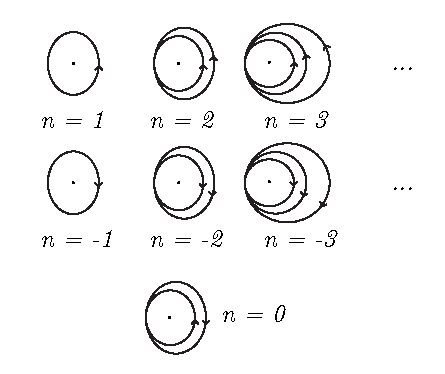
\includegraphics[scale = 1.2]{windingnumber}
\end{figure}
\end{frame}

%%%%%%%%%%%%%%%%%%%%%%%%%%%%%%%%%%%%%%%%%%%%%%%%%%%%%%%%%%%%%%%%%%%%%%%%%%%%%%%%
%%%%%%%%% CONCLUSIONI %%%%%%%%%%%%%%%%%%%%%%%%%%%%%%%%%%%%%%%%%%%%%%%%%%%%%%%%%%
\begin{frame}
\frametitle{Conclusioni}
Monopolo magnetico spiega:
\begin{itemize}
   \item Quantizzazione della carica dell'elettrone (osservata sperimentalmente)
   \item Simmetria rotta tra campi $\vec B$ ed $\vec E$ ristabilita
      \begin{equation*} \begin{aligned}
      \nabla \cdot \vec E & = 4\pi\rho & \nabla \cdot \vec B & = 4\pi\rho_g
      \end{aligned}\end{equation*}
   \item e molto altro...
\end{itemize}

\begin{center}\Large
   Se non esistono, perchè?
\end{center}
\end{frame}

\end{document}
